\documentclass[10pt]{article}
\usepackage[a4paper,margin=18mm]{geometry}
\usepackage{amsmath,amssymb,booktabs,graphicx,microtype}
\usepackage[hidelinks]{hyperref}
\usepackage[numbers,sort&compress]{natbib}
\usepackage{enumitem}
\setlist{nosep,leftmargin=*}
\title{MedTAWS-GRPO: Workflow-Tree Search and Group-Relative Prompt-Trajectory Alignment for Interactive 3D Medical Image Segmentation}
\author{Anonymous Author(s)\\Anonymous Institution}
\date{}
\begin{document}
\maketitle
\begin{abstract}
Promptable three-dimensional medical segmentation models expose two coupled sources of downstream error: the inference workflow that converts interactions into predictions, and the model parameters that determine how the prompts are interpreted. Most adaptation studies optimize only one of these components and consequently confound workflow engineering with weight adaptation. We introduce \textbf{MedTAWS-GRPO}, a two-level framework that separates and then connects discrete workflow optimization and continuous model adaptation. MedTAWS (Medical Tree-guided Adaptive Workflow Search), built on AFlow, represents executable segmentation workflows as nodes and uses a stochastic upper-confidence-bound policy to balance validation quality against under-explored branches. Every evaluation is tied to an immutable objective, budget, fold, and provenance receipt. The training component performs GRPO-style group-relative alignment over multiple corrective prompt trajectories from the same volume. It normalizes a morphology-aware overlap reward within each trajectory group and updates the prompt encoder and mask decoder under reference-model and supervised anchors. A retrospective development study on postoperative glioma resection-cavity segmentation shows that group size four with a 0.05 supervised anchor improves mean Dice from 0.57283 for a matched supervised model to 0.58932 across two seeds. The 0.01649 gain is a development signal, not a confirmatory result: the historical cohort contains longitudinal subject overlap, uses oracle corrective clicks and ground-truth-centered crops, and has not been evaluated jointly with MedTAWS on a subject-disjoint holdout. Negative cross-target and reward-shaping results further show that the benefit is target-specific. These findings establish an auditable optimization framework and identify the experiments required for a valid confirmatory study without overstating current clinical generalization.

\textbf{Keywords:} interactive medical image segmentation; SAM-Med3D; workflow search; group-relative optimization; reinforcement learning; postoperative glioma

\end{abstract}
\begin{figure}[t]\centering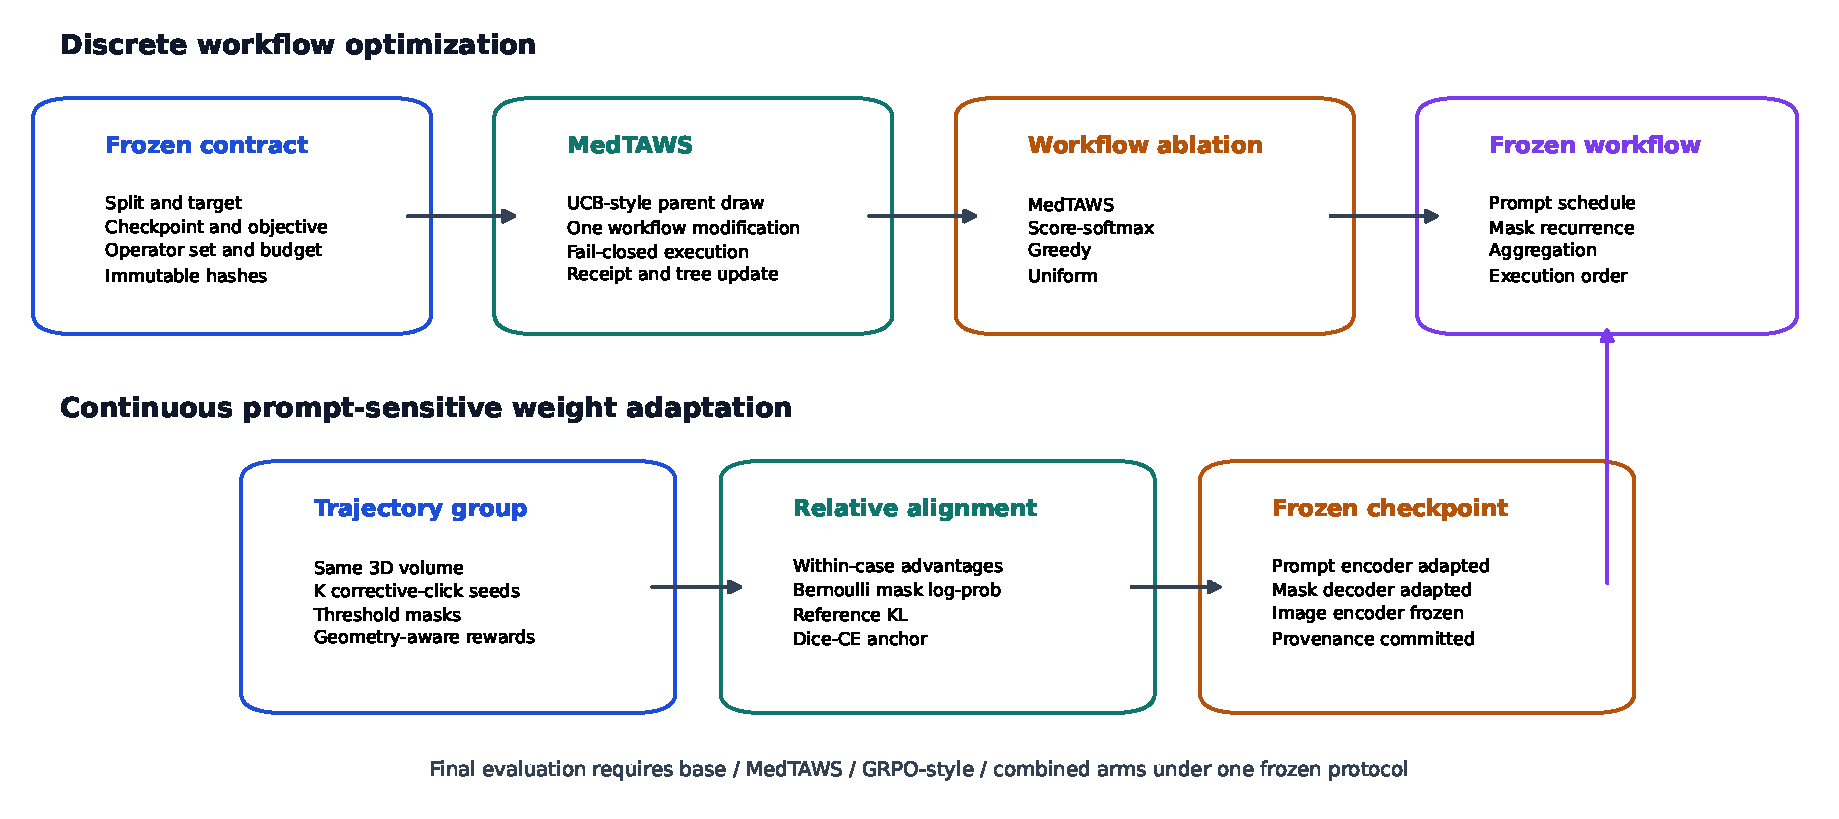
\includegraphics[width=\linewidth]{figures/framework_overview.pdf}\caption{Overview of the two-level MedTAWS-GRPO framework.}\end{figure}
\section{Introduction}
Post-treatment glioma segmentation is difficult because surgery and therapy alter the anatomy that a model must delineate. Resection cavities, enhancing tissue, non-enhancing core, and treatment-related hyperintensity can be small, fragmented, low contrast, and variable across longitudinal examinations. The BraTS 2024 post-treatment challenge formalized these regions and emphasized lesion-wise evaluation on held-out data \cite{brats2024}. In this setting, a high-capacity segmentation backbone alone does not determine performance. Input preparation, prompt trajectories, recurrent-mask handling, aggregation, and parameter adaptation all affect the final mask.

Promptable foundation models provide a useful interface for this problem. Segment Anything introduced a general prompt-conditioned segmentation formulation \cite{sam}, while MedSAM and SAM-Med3D adapted this idea to medical images and volumetric inputs \cite{medsam,sammed3d}. A promptable model can incorporate expert corrections without retraining for every case. However, its apparent downstream accuracy is highly sensitive to the interaction protocol. A first click sampled from a target, an error-driven corrective click, an accumulated point set, and a recurrent low-resolution mask are not interchangeable experimental conditions. Optimizing these choices on validation data can improve a workflow even when the weights are frozen, but uncontrolled search can also leak label information, overspend an evaluation budget, or turn a development set into a de facto test set.

Weight adaptation introduces a second optimization problem. Conventional supervised fine-tuning treats each simulated prompt trajectory independently and minimizes a voxel-wise or overlap loss. It does not explicitly compare different trajectories for the same volume, even though trajectory quality can vary substantially. Group Relative Policy Optimization (GRPO) estimates a baseline from a group of outputs rather than a learned critic \cite{deepseekmath}. This makes its central idea attractive for segmentation, where several prompt trajectories can be evaluated by deterministic geometric rewards. Directly transferring language-model GRPO is nevertheless inappropriate: a dense mask is not a token sequence, the action space is extremely large, and deterministic thresholded masks do not constitute sampled Bernoulli actions.

We address both levels with MedTAWS-GRPO. The outer MedTAWS component searches over executable promptable-segmentation workflows. It is derived from AFlow \cite{aflow} but uses a segmentation-specific, fail-closed evaluator and a stochastic UCB-style parent policy. The inner component performs \textbf{GRPO-style group-relative prompt-trajectory alignment}. Several corrective-click trajectories are generated for one training volume; their rewards are normalized within the group; and the prompt encoder and mask decoder are updated with a group-relative surrogate, a fixed-reference Bernoulli KL term, and a supervised Dice-CE anchor.

The contributions are threefold:

\begin{enumerate}
\item We formulate promptable 3D medical segmentation as a two-level optimization problem over an executable workflow and model parameters, separating inference-policy gains from weight-adaptation gains.
\item We introduce MedTAWS, a seeded stochastic UCB workflow-tree policy with strict objective, provenance, budget, and label-boundary validation. The implementation is deliberately described as UCB-guided workflow search rather than standard Monte Carlo tree search.
\item We adapt group-relative optimization to corrective 3D mask trajectories and report both positive and negative development evidence. The matched two-seed RC result is positive but small, while cross-target and reward-shaping experiments expose the limits of the current formulation.
\end{enumerate}
\section{Related Work}
\subsection{Promptable and interactive segmentation}
Interactive segmentation uses points, scribbles, boxes, or prior masks to refine predictions. DeepIGeoS showed that user interactions can guide 2D and 3D medical segmentation through geodesic encodings and iterative refinement \cite{deepigeos}. RITM demonstrated the importance of iterative training and recurrent mask guidance for click-based segmentation \cite{ritm}, and SimpleClick obtained strong interactive results with a plain vision-transformer backbone \cite{simpleclick}. SAM generalized promptable segmentation at large scale \cite{sam}. MedSAM trained a medical variant on more than one million image-mask pairs \cite{medsam}, while SAM-Med3D constructed a fully 3D promptable model and volumetric training corpus \cite{sammed3d}. Our work does not propose a new image encoder. It optimizes the workflow surrounding SAM-Med3D and adapts the prompt-sensitive modules using relative trajectory quality.

\subsection{Automated workflow search}
AFlow casts agentic workflow construction as search over code-represented workflows and uses execution feedback to improve candidates \cite{aflow}. Medical segmentation differs from the language benchmarks for which AFlow was developed: the evaluator is GPU-intensive; spatial labels must never enter the inference workflow; case and subject boundaries matter; and repeated validation access can invalidate clinical claims. MedTAWS retains AFlow's central workflow-generation insight but adds deterministic canonicalization, fixed evaluation contracts, fail-closed receipts, and search-budget accounting. Its parent-selection implementation uses direct-child counts as a visit proxy and does not contain rollouts or ancestor value backup. It is therefore not standard MCTS.

\subsection{Group-relative optimization}
PPO stabilizes policy updates with a clipped importance-ratio objective \cite{ppo}. DeepSeekMath introduced GRPO, which replaces a learned value model with a group-derived baseline \cite{deepseekmath}. This critic-free relative comparison is particularly appealing when multiple outputs for the same input can be scored by a rule-based reward. In our setting, the group consists of stochastic prompt trajectories rather than language completions. The current implementation computes deterministic threshold masks and performs one update from the same forward pass. Its importance ratio is one in the forward evaluation, so the method should be understood as GRPO-style group-relative mask alignment, not as a complete reproduction of PPO or language-model GRPO.

\subsection{Post-treatment glioma segmentation}
The BraTS 2024 post-treatment task defines four atomic regions: enhancing tissue, surrounding non-enhancing FLAIR hyperintensity, non-enhancing tumor core, and resection cavity \cite{brats2024}. Fully automatic systems commonly use self-configuring or large-kernel 3D backbones such as nnU-Net and MedNeXt \cite{nnunet,mednext}. Their four-modal, automatic, lesion-wise scores are not directly comparable to a single-modal, oracle-click, binary interactive protocol. We therefore do not place external automatic-segmentation values in the same quantitative table as our retrospective interactive study.

\section{Method}
\subsection{Problem formulation}
Let \(x\in\mathbb{R}^{1\times H\times W\times D}\) be a 3D MR volume, \(y\in\{0,1\}^{H\times W\times D}\) a binary target mask, and \(\tau=(p_1,\ldots,p_T)\) a sequence of positive or negative point prompts. A promptable model \(f_\theta\) produces logits

\[
z=f_\theta(x,\tau,m_{t-1}), \qquad \hat y=\mathbb{1}[\sigma(z)>0.5],
\]
where \(m_{t-1}\) is an optional recurrent low-resolution mask. We distinguish two decision variables. The \textbf{workflow} \(w\) specifies prompt construction, point accumulation, recurrent-mask use, candidate aggregation, and execution order. The model parameters \(\theta\) specify the prompt encoder and mask decoder behavior. Development performance is

\[
J(w,\theta;\mathcal D_{dev})=\frac{1}{|\mathcal D_{dev}|}
\sum_{(x,y)\in\mathcal D_{dev}}\operatorname{Dice}
\left(\mathcal E(w,f_\theta,x),y\right),
\]
where \(\mathcal E\) is a controlled evaluator. MedTAWS searches over \(w\) with \(\theta\) fixed. Group-relative alignment updates \(\theta\) under a frozen workflow. This separation allows each improvement to be attributed to one optimization level before a final coupled evaluation.

\subsection{MedTAWS workflow representation}
MedTAWS represents each successfully evaluated workflow as a node

\[
n_i=(w_i,q_i,\mathcal P_i,C_i^+,C_i^-),
\]
where \(q_i\) is the frozen validation objective, \(\mathcal P_i\) is immutable provenance, and \(C_i^+\) and \(C_i^-\) are improving and non-improving direct children. The provenance binds the dataset-manifest hash, checkpoint hash, code hash, workflow hash, operator-set hash, optimizer-prompt hash, objective hash, fold identifier, LLM provider and model, and search seed. A node is rejected if any required field is absent or inconsistent with the search contract.

The proposal generator receives the parent workflow and structured parent experience, then applies one conceptual modification from the frozen operator set. The workflow payload cannot include a field whose name denotes ground truth, labels, or segmentation paths. Ground truth is visible only inside the evaluator after inference, where it is used to compute the frozen objective. A successful evaluation returns a one-time receipt. Duplicate workflows, invalid receipts, out-of-contract objectives, and over-budget calls fail closed rather than being assigned a numeric score.

\subsection{Stochastic UCB parent selection}
For node \(i\), the implementation defines a direct-child visit proxy

\[
v_i=1+|C_i^+|+|C_i^-|.
\]
Given \(K\) candidate nodes, its utility is

\[
U_i=100\left[q_i+c\sqrt{\frac{\log(1+\sum_{j=1}^{K}v_j)}{v_i}}\right].
\]
Before any candidate has been expanded, the selection falls back to \(U_i=100q_i\). Utilities are converted to a score distribution and mixed with uniform exploration:

\[
s_i=\frac{\exp(\alpha U_i)}{\sum_j\exp(\alpha U_j)},\qquad
p_i=\frac{\lambda}{K}+(1-\lambda)s_i.
\]
The frozen defaults are \(c=0.08\), \(\alpha=0.2\), and \(\lambda=0.3\). A seeded categorical draw selects the parent. The complete draw record includes the ordered candidates, visit proxies, utilities, probabilities, selected node, objective, and seed. MedTAWS is compared under identical logical backend budgets with score-softmax, greedy, and uniform parent policies. The intended search statistics are final best score, best-so-far area under the evaluation-budget curve, valid-workflow rate, model forwards, LLM calls, wall time, and peak memory.

\subsection{Group-relative prompt-trajectory alignment}
For a training pair \((x,y)\), we generate \(K\) corrective prompt trajectories \(\tau_i\) by varying the trajectory seed. Each trajectory produces logits and a deterministic binary mask:

\[
z_i=f_\theta(x,\tau_i),\qquad a_i=\mathbb{1}[\sigma(z_i)>0.5].
\]
The historical RC configuration uses the reward

\[
\begin{split}
R_i ={}& 1.2\,\operatorname{Dice}(a_i,y)
-0.25\,\mathbb{1}[|y|>0\land|a_i|=0]\\
&-0.05\left|\log\frac{|a_i|+1}{|y|+1}\right|
-0.02\,\mathbb{1}[C_i>1]\log C_i,
\end{split}
\]
where \(C_i\) is the number of connected components in \(a_i\). The target weight 1.2 compensates for the weak RC target in the historical mixed-target development code. Rewards are normalized only within trajectories from the same volume:

\[
A_i=\frac{R_i-\bar R}{\operatorname{Std}(R)+\epsilon}.
\]
For the threshold mask \(a_i\), the mean voxel-wise Bernoulli log-probability is

\[
\ell_i(\theta)=\frac{1}{|\Omega|}\sum_{u\in\Omega}
\left[a_{iu}\log p_{iu}+(1-a_{iu})\log(1-p_{iu})\right],
\quad p_i=\sigma(z_i).
\]
The code expresses the group-relative term with a PPO-style clipped ratio

\[
\mathcal L_{rel}=-\frac1K\sum_i
\min(r_iA_i,\operatorname{clip}(r_i,1-\varepsilon,1+\varepsilon)A_i),
\]
and adds a fixed-reference Bernoulli KL term and a supervised Dice-CE anchor:

\[
\mathcal L=\mathcal L_{rel}
+\beta D_{KL}^{Bern}(p_\theta\Vert p_{ref})
+\eta\mathcal L_{DiceCE}.
\]
The main configuration uses \(K=4\), \(\varepsilon=0.2\), \(\beta=0.02\), and \(\eta=0.05\). The prompt encoder and mask decoder are trainable; the image encoder and reference model are frozen. Importantly, the implementation sets the old log-probability to a detached copy of the same forward pass and performs a single update. Thus \(r_i=1\) in the forward evaluation and clipping does not become active. Gradient weighting still follows the group-normalized advantage, but this is not a multi-epoch old-policy PPO update.

\subsection{Coupled protocol}
The complete framework follows four stages:

\begin{enumerate}
\item Freeze the data split, target definition, interaction protocol, checkpoint, objective, operator set, and evaluation budget.
\item With the base checkpoint fixed, compare MedTAWS, score-softmax, greedy, and uniform search on development subjects under identical budgets.
\item Freeze the selected workflow, then compare supervised fine-tuning and group-relative alignment using identical cases, epochs, seeds, initialization, and evaluation code.
\item Before opening a confirmatory holdout, freeze one base, one MedTAWS-only, one GRPO-style-only, and one combined checkpoint-workflow pair. Evaluate each exactly once.
\end{enumerate}
The historical project completed stages 2 and 3 in separate legacy protocols, but not a valid joint stage 4. Section 4 therefore distinguishes implemented method evidence from confirmatory evidence.

\section{Experimental Design}
\subsection{Dataset and evidence tiers}
We use the BraTS 2024 post-treatment adult glioma resource \cite{brats2024}. The historical GRPO-style development study was constructed from 200 scans corresponding to only 39 longitudinal subjects. It used the T1 contrast-enhanced channel and the raw resection-cavity label (label 4) as a binary target. Volumes were transformed to canonical orientation and cropped or padded to \(128^3\) around a ground-truth-derived target center.

The historical split is not subject-disjoint. All 16 validation subjects also appear in the training partition through other longitudinal scans. Consequently, every number in Sections 5.1--5.5 is labeled \textbf{retrospective development evidence}. It cannot support a patient-generalization, current T1ce residual-tumor, fully automatic, or state-of-the-art claim. No sealed test result is reported.

The current full-data protocol contains 1,350 scans and uses an 80/20 case split, but GRPO-style training and MedTAWS have not yet been run jointly under the corrected subject-clean target protocol. Those experiments are specified in Section 6.4 and intentionally remain absent from the numerical tables.

\subsection{Historical interaction protocol}
Each training rollout used five simulated corrective clicks. The initial interaction was sampled from the target. Later interactions were sampled from error regions, with positive clicks from false negatives and negative clicks from false positives. A recurrent low-resolution mask was passed between iterations. In the historical trainer, only the current point, rather than the accumulated point set, was sent at each recurrent step. These oracle interactions quantify an interactive upper-bound setting and do not represent automatic segmentation.

\subsection{Training configuration}
Both supervised and group-relative models were initialized from the same four-case supervised M0 checkpoint. The image encoder was frozen. The prompt encoder and mask decoder contained 7,584,304 trainable parameters out of 100,509,232 total parameters. We used AdamW with learning rate \(2\times10^{-5}\), weight decay \(10^{-4}\), batch size one, mixed precision, and two seeds (2026 and 2027). The matched full-development comparison used 118 training scans, 16 validation scans, and 10 epochs.

\subsection{Evaluation}
Hard Dice is

\[
\operatorname{Dice}(a,y)=\frac{2|a\cap y|}{|a|+|y|}.
\]
The historical audit reports the mean over 16 validation scans and four trajectories per scan. It is therefore a 64-rollout mean, not a patient-balanced macro average. Checkpoints were selected by validation Dice during training and reloaded for a separate hard-mask audit. Because only two seeds are available and the validation subjects overlap training, we report the seed values and arithmetic mean without a significance claim.

\subsection{Baselines and ablations}
The matched baseline is supervised decoder-side adaptation with Dice-CE loss. Group-relative ablations vary group size and supervised-anchor strength. Additional diagnostic variants include pairwise preference loss, center and surface rewards, boundary-weighted anchoring, hard-case curriculum, logit noise, rank advantages, mixed-soft rewards, advantage-weighted regression, and a corrective objective that removes negative group-relative pressure. Cross-target checks use enhancing-tumor and tumor-core binary targets.

\section{Results}
\subsection{Matched supervised comparison}
Table 1 contains the only same-size, same-epoch, two-seed supervised comparison. GRPO-style alignment improves mean Dice by 0.01649. The margin is uneven: +0.02961 for seed 2026 and +0.00337 for seed 2027. The result supports a small development-set benefit, not a robust generalization claim.

\begin{table}[t]
\centering
\small
\caption{Table 1. Retrospective RC development result. The split contains longitudinal subject overlap.}
\resizebox{\linewidth}{!}{%
\begin{tabular}{lrrrrrr}
\toprule
Method & Train/Val & Epochs & Seed 2026 & Seed 2027 & Mean Dice & Delta \\
\midrule
Supervised Dice-CE & 118/16 & 10 & 0.56454 & 0.58113 & 0.57283 & - \\
GRPO-style, K=4, anchor=0.05 & 118/16 & 10 & \textbf{0.59415} & \textbf{0.58450} & \textbf{0.58932} & +0.01649 \\
\bottomrule
\end{tabular}%
}
\end{table}
\subsection{Data and training-length trend}
Table 2 records the development progression of the selected group-relative configuration. Performance increases with more scans and longer training. These rows do not isolate a causal variable because sample count and epoch count change across the sequence.

\begin{table}[t]
\centering
\small
\caption{Table 2. GRPO-style RC development progression; values are two-seed reload-audit means.}
\resizebox{\linewidth}{!}{%
\begin{tabular}{lrrr}
\toprule
Training scans & Validation scans & Epochs & Mean Dice \\
\midrule
32 & 16 & 5 & 0.44198 \\
64 & 16 & 5 & 0.51247 \\
96 & 16 & 5 & 0.53777 \\
118 & 16 & 5 & 0.54698 \\
118 & 16 & 8 & 0.56923 \\
118 & 16 & 10 & \textbf{0.58932} \\
\bottomrule
\end{tabular}%
}
\end{table}
\subsection{Group size and anchor ablation}
At 32 training scans, group size two with anchor 0.10 does not exceed the supervised baseline. Increasing the group to four improves Dice for both anchor values, and reducing the anchor from 0.10 to 0.05 gives the best two-seed result. This pattern is consistent with the intended mechanism: a larger within-case comparison set provides a more informative relative ordering, while an excessively strong supervised term suppresses the relative update.

\begin{table}[t]
\centering
\small
\caption{Table 3. Two-seed RC ablation at 32 training scans and 5 epochs.}
\resizebox{\linewidth}{!}{%
\begin{tabular}{lrrr}
\toprule
Objective & Group size & Supervised anchor & Mean Dice \\
\midrule
Supervised Dice-CE & - & 1.00 & 0.42431 \\
GRPO-style & 2 & 0.10 & 0.42269 \\
GRPO-style & 4 & 0.10 & 0.43770 \\
GRPO-style & 4 & 0.05 & \textbf{0.44198} \\
\bottomrule
\end{tabular}%
}
\end{table}
\subsection{Negative ablations and target specificity}
Table 4 summarizes diagnostic variants. Most intuitive reward extensions do not improve the selected formulation. Pairwise objectives discard dense reward magnitude; coarse center constraints and explicit surface terms can dominate small structures; and replacing negative relative pressure with supervised correction moves the update back toward ordinary fine-tuning. The single-seed mixed-soft value is only 0.00203 above its same-seed reference and was not replicated.

\begin{table}[t]
\centering
\small
\caption{Table 4. Diagnostic RC ablations. Two-seed values are marked; all others are single-seed.}
\resizebox{\linewidth}{!}{%
\begin{tabular}{lrr}
\toprule
Variant & Reload Dice & Evidence \\
\midrule
Selected GRPO-style, K=4, anchor=0.05 & 0.44198 & two-seed mean \\
Pure pairwise & 0.41865 & two-seed mean \\
GRPO + pairwise & 0.42739 & two-seed mean \\
Center reward & 0.42915 & two-seed mean \\
Anchor/KL schedule & 0.43694 & two-seed mean; seed reversal \\
Surface reward & 0.42378 & single seed \\
Boundary-weighted anchor & 0.40737 & single seed \\
Hard-case curriculum & 0.42267 & single seed \\
Rank advantage & 0.44234 & single seed; reference 0.44541 \\
Mixed-soft reward & 0.44743 & single seed; reference 0.44541 \\
GRPO + AWR, best setting & 0.43841 & single seed \\
Corrective GRPO, best setting & 0.43740 & single seed \\
\bottomrule
\end{tabular}%
}
\end{table}
The benefit also fails to transfer to two related binary targets. For enhancing tumor, supervised and GRPO-style means are 0.39315 and 0.38590, respectively. For tumor core they are 0.41736 and 0.41266. These reversals indicate that the RC reward weights and trajectory distribution cannot be assumed to generalize to smaller or differently structured targets.

\subsection{Historical MedTAWS signal}
Legacy workflow search produced an ET validation candidate improvement from 0.31247 to 0.32748. On a broader historical evaluation, the WT/TC/ET macro changed from 0.46988 to 0.47341, whereas an all-label case-weighted score decreased from 0.50972 to 0.50748. These values demonstrate that executable UCB-guided search ran end to end and could discover target-specific candidates, but they do not establish consistent multi-target benefit.

The legacy search used scan-level partitions, oracle prompts, mixed objectives, unequal stochastic inference counts across some rounds, and no equal-budget multi-seed comparison against greedy or random selection. A later equal-budget implementation was correctly withdrawn after discovering that four SAM-Med3D mask tokens had been misinterpreted as semantic classes. We therefore exclude MedTAWS numbers from the main comparative tables and make no claim that it outperforms greedy selection.

\section{Discussion}
\subsection{Two optimization levels should be separated}
The central methodological point is that workflow optimization and weight adaptation answer different questions. MedTAWS asks which executable interaction policy should surround a fixed model. Group-relative alignment asks how a model should rank and reinforce prompt trajectories under a fixed workflow. Reporting only a final Dice after changing both makes attribution impossible. A four-arm final study - base, MedTAWS only, GRPO-style only, and combined - is necessary to measure their individual and interaction effects.

\subsection{Why group-relative alignment can help}
The matched RC experiment suggests that comparing trajectories within the same volume can recover a small improvement after a strong supervised model has already learned most of the task. Within-case normalization removes much of the case-difficulty scale and directs the update toward which interaction trajectory is better for that volume. The group-size ablation supports this interpretation: four trajectories are more useful than two. The fixed reference and Dice-CE anchor constrain the model from exploiting reward artifacts.

The observed gain is not large. Expanding from 32 to 118 training scans accounts for much more of the absolute improvement than replacing supervised training with the group-relative objective. This distinction matters for method claims. The evidence supports a modest optimization benefit after controlling for data and epochs, not a dramatic advantage of reinforcement learning over supervision.

\subsection{Why several extensions fail}
Negative results clarify the useful signal. Pairwise best-versus-worst losses compress a continuous geometric reward into a binary ordering. Center and connectedness constraints can reward a plausible global shape while missing small RC boundaries. Surface rewards can become unstable at low resolution. A corrective objective that applies relative pressure only to positive advantages underperforms the original positive-negative push, suggesting that poor trajectories still provide useful contrastive information. ET and TC reversals show that reward coefficients and click distributions must be target-conditioned.

\subsection{Required confirmatory experiment}
A valid confirmatory study must be rerun from the corrected full cohort. Subjects, rather than scans, must define train, validation, and test partitions. The final target must be frozen as either raw RC or a clearly specified residual-tumor union. The interaction protocol must state whether it is simulated-oracle, human-interactive, or fully automatic. The initial click, subsequent FN/FP sampling, point accumulation, recurrent mask, crop rule, and click count must be identical across methods.

Before opening the holdout, four configurations must be frozen: base SAM-Med3D, MedTAWS only, matched supervised or GRPO-style adaptation only, and the combined method. MedTAWS, score-softmax, greedy, and uniform policies require identical workflow-evaluation budgets and at least three search seeds. Model adaptation requires at least three training seeds and a matched supervised control at the same data size and epoch budget. The holdout should report subject-balanced Dice, IoU, HD95, per-click Dice curves, confidence intervals, paired tests, inference time, model forwards, and memory. External automatic BraTS systems should appear only in a separate table with an explicit protocol mismatch, or not at all.

\section{Limitations}
This study has seven material limitations. First, the retrospective 200-scan dataset contains only 39 longitudinal subjects and has complete train-validation subject overlap. Second, the RC task uses one T1 contrast-enhanced modality and cannot be compared with four-modal automatic BraTS results. Third, ground-truth-centered crops and simulated error clicks create an oracle interactive setting. Fourth, the reported Dice is averaged over scans and trajectories rather than subjects. Fifth, the group-relative implementation uses deterministic threshold masks, a same-forward detached old log-probability, and a single update; it is GRPO-style alignment rather than standard PPO/GRPO. Sixth, GRPO-style alignment is positive only on RC and negative on ET and TC. Seventh, MedTAWS and group-relative adaptation have not been jointly evaluated under a subject-disjoint protocol. These limitations preclude a state-of-the-art or clinical-generalization claim.

\section{Conclusion}
We presented MedTAWS-GRPO, a reproducibility-first framework for optimizing both the executable workflow and prompt-sensitive weights of a 3D interactive segmentation model. MedTAWS contributes seeded stochastic UCB workflow-tree search with strict provenance and budget enforcement. The training component contributes within-volume, group-relative prompt-trajectory alignment with geometric rewards, reference regularization, and supervised anchoring. A retrospective RC experiment shows a small matched improvement of 0.01649 Dice, while extensive negative ablations and cross-target reversals constrain the claim. The framework is implemented, but the decisive subject-disjoint joint evaluation remains future experimental work. Freezing that protocol before holdout access is essential for converting the current development signal into defensible evidence.

\section{Data and Code Availability}
The method is implemented in the project modules \texttt{medtaws/search.py}, \texttt{medtaws/ablation.py}, and \texttt{scripts/train\_sammed3d\_grpo.py}. The BraTS data are governed by the challenge access terms and are not redistributed. A release should include frozen manifests, configuration files, checkpoint and workflow hashes, search receipts, per-case metrics, and the exact code revision used for confirmatory evaluation.

\bibliographystyle{unsrtnat}
\bibliography{references}
\end{document}
